\section*{17-05 - Galassie}
Il primo a capire il motivo della distribuzione asimmetrica della Via Lattea fu William Herschel. Assunse che le stelle fossero tutte simili a Sirio, quindi con la stessa luminosità intrinseca, ed il confronto tra la luminosità intrinseca e quella apparente permetteva di ricostruirne le distanze. Ovviamente questo è un approccio molto grossolano poiché le stelle non hanno la stessa luminosità. Fece l'errore di considerare il sole al centro dela galassia. Nonostante ciò, Herschel riuscì a rendersi conto che la galassia ha una distribuzione schiacciata e non a simmetria sferica. Qualche anno dopo questo modello venne raffinato da Kepteyn confermando che l'altezza di scala dovesse essere piccola rispetto alla sua estensione. (pag 4/151 galassie) Successivamente Shapley studiò gli ammassi globulari per cercare di capire la struttura della galassia. Studiando la distribuzione geometrica di questi oggetti Shapley si rese conto di una distribuzione degli ammassi globulari nella zona del Sagittario. Si rese conto dell'apparenza di questo fenomeno e lo tradusse considerando il Sole posto in una zona periferica. Studiando la distanza da noi degli ammassi, ricostruì le dimensioni della galassia e la distanza dal centro. Oggi sappiamo le distanze del Sole dal centro della galassia ($\sim 8\um{kpc}$, circa $2/3$ del diametro). Per capire queste distanze Shapley utilizzò un particolare tipo di stelle variabili, le Lyrae. Qualche tempo prima un altro tipo di variabili furono usate da Henrietta Leavitt, le Cefeidi classiche. Un obiettivo di ricerca della scienziata era capire se esistesse e quale fosse la relazione tra periodo e luminosità delle stelle variabili. Ebbe l'intuizione di studiare le cefeidi della Nube di Magellano, dato che, essendo in una zona ristretta del cielo, erano tutte più o meno alla stessa distanza da noi. Quindi la differenza tra magnitudine apparente tra due cefeidi riflette una differenza tra magnitudine assoluta. Leavitt scoprì una relazione lineare tra il logaritmo della luminosità ed il logaritmo del periodo. Quindi una volta calibrata questa relazione, è possibile scoprire la luminosità intrinseca degli oggetti e di conseguenza trovare le distanze di questi. A tutt'oggi le cefeidi classiche sono la principale candela campione primaria nella scala di distanze extragalattiche. La principale stima della costante di Hubble si basa proprio sulla relazione periodo-luminosità delle cefeidi. Shapley fu uno dei primi a calibrare questa relazione e quello che emerse fu appunto che il Sole fosse periferico nella galassia e che questa abbia una struttura a disco con un alone di ammassi globulari distribuiti attorno al disco ed un bulge al centro della galassia. Il disco ha un diametro di circa 15 kpc, mentre risulta spesso 50 pc per le stelle di tipo O e B mentre 200 pc per quelle di tipo K. L'altezza cambia a seconda del tipo spettrale delle stelle perché le stelle massicce vivono poco e hanno poco tempo per spostarsi, mentre quelle piccole hanno avuto molto tempo per diffondersi. (pag. 13/151 galassie). Sul disco le stelle hanno metallicità maggiore ed età diverse.\\
Come mai Herschel e Kapteyn hanno fatto l'errore di considerare il Sole al centro della galassia? Il motivo è che non ci sono solo stelle, ma anche una cosa che loro non conoscevano: il mezzo interstellare. Ci siamo resi conto della sua esistenza per la prima volta nel 1930 quando Trumpler, studiando gli ammassi aperti, si rese conto che dovesse esistere un qualche tipo di mezzo che assorbisse la luce. Lui fece l'ipotesi che, come ordine di grandezza, le dimensioni degli ammassi aperti fossero confrontabili, e quindi misurando la dimensione angolare avrebbe avuto una misura delle distanze. Trumpler si mise a confrontare la magnitudine apparente con la dimensione angolare. Si aspettava che al diminuire della dimensione angolare (aumentare la distanza) la luminosità apparente diminuisse come $1/R^2$ (essendoci il vuoto) e quindi, sapendo che $(m-M)=-5+5\log(d)$, Trumpler si rese conto che la magnitudine apparente diminuisse più rapidamente e capì che ciò fosse dovuto ad un mezzo che assorbiva la luce. Quindi alla relazione di prima va aggiunto un termine di estinzione e si ha 
\[
    (m-M)=-5+5\log(d)+A_{\lambda}, \ A_{\lambda}>0.
\]
Guardando nel visibile $A_V \approx 1.5 d,\ [d]=\um{kpc}$. Dato che il termine di estinzione dipende dalla lunghezza d'onda, si produce un effetto sul colore della sorgente. A causa del mezzo si avrà un'estinzione diversa per banda diversa. La differenza $(B-V)-(B-V)_0=E(B-V)$ prende il nome di arrossamento (reddening). La forma del continuo dello spettro viene modificata, ed in particolare l'estinzione nel B è maggiore dell'estinzione del V, da cui arrossamento. Nel caso del disco della nostra galassia $E(B-V)\approx 0.5 d,\ [d]=\um{kpc}$. Prendendo il rapporto
\[
\frac{A_\lambda}{E(B-V)}
\]
questo non dipende dalla distanza. Sul libro vediamo un grafico del rapporto in funzione di lambda in cui si vede una zona con un picco a circa 2200 \AA e, lontano dal picco, l'estinzione scala come $1/\lambda$. Queste relazioni ci dicono che ciò che produce l'arrossamento è polvere (grani macroscopici, della frazione di micron), che produce l'estinzione e ci permette di dire che un contributo grosso è dovuto alla grafite ed un altro ai silicati.\\
Anche la polvere si trova principalmente sul disco. A produrre la polvere sono le stelle nell'inviluppo delle giganti rosse, ma anche l'esplosione di supernova.\\
Si capisce quindi che le stelle non vivono nel vuoto, ma ci deve essere un mezzo interstellare. All'inizio si vide la parte di polvere ma poi ci si rese conto che questa non fosse la parte dominante in massa. C'è anche una componente gassosa, che si riuscì a capire osservando negli spettri. Negli spettri delle stelle si osservarono delle righe di assorbimento di elementi non prodotti nella fotosfera della stella ma bensì nel mezzo che ci separa dalla stessa. Ci si rese conto della cosa poiché, come sappiamo, il profilo di riga assume un profilo gaussiano dovuto all'agitazione termica (doppler). Nel caso della fotosfera ci aspettiamo larghezze molto più grandi a causa della temperatura maggiore, mentre nello spettro si trovarono righe sottili compatibili con gli allargamenti termici di temperature molto basse. La prova del nove si ebbe osservando sistemi binari: le righe delle stelle si muovevano avanti e indietro per effetto doppler ma chiaramente quelle del mezzo no. Si comprese quindi che oltre alla polvere fosse presente un mezzo gassoso, che veniva all'inizio studiato solo nell'assorbimento prodotto osservando le stelle. Non si riusciva ad osservare l'emissione del mezzo in se poiché è molto freddo ($T\sim(80\div100)\um{K}$). A queste temperature ci aspettiamo che l'idrogeno sia nel fondamentale, quindi nelle bande del visibile non ci aspettiamo un emissione da parte del mezzo. \\
\begin{figure}[t!]
    \centering
    \resizebox{.8\columnwidth}{!}{%
        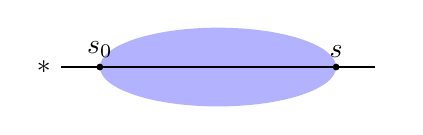
\begin{tikzpicture}
            \fill[blue!30] (0,0) ellipse (1.5 and 0.5);
            \draw (-2,0) -- (2,0) node[left, pos=0]{$*$} node[right,pos=1]{$\text{\lateraleye}$};
            \filldraw[black] (-1.5,0) circle (1pt) node[above] {$s_0$};
            \filldraw[black] (1.5,0) circle (1pt) node[above] {$s$};
        \end{tikzpicture}
    }
    \caption{Luce della stella che passa attraverso il mezzo interstellare.}
    \label{fig:tralenubi}
\end{figure}
Siamo a queste temperature. Consideriamo la sezione d'urto di assorbimento di un atomo in generale:
\[
\sigma = \frac{e^2}{4\epsilon_0m_ec} f \text{ (si trova sul libro)}
\]
Sappiamo inoltre che il coefficiente di assorbimento è legato alla sezione d'urto:
\[
    \alpha_\nu= n\sigma\Phi(\Delta \nu)=\frac{e^2}{4\epsilon_0 M_e c}nf\Phi(\Delta \nu), \quad \int \Phi(\Delta \nu)d\nu = 1.
\]
Noto il coefficiente di assorbimento, possiamo calcolare la profondità ottica, che è ciò che vogliamo ottenere
\[
    \tau_\nu = \int_{s_0}^{s} \alpha(s')ds' = \int_{s_0}^{s}\frac{e^2}{4\epsilon_0 M_e c}nf\Phi(\Delta \nu) ds'= \frac{e^2}{4\epsilon_0 M_e c}f\Phi(\Delta \nu)\int_{s_0}^{s}nds'.
\]
L'ultimo integrale si indica di solito con $N=\int_{s_0}^{s}nds'$ e prende il nome di densità di colonna (degli atomi che assorbono i fotoni con la frequenza della riga). Quindi
\[
    \tau_\nu = \frac{e^2}{4\epsilon_0 M_e c}f\Phi(\Delta \nu) N.
\]
Vogliamo calcolare la larghezza equivalente. Noi sappiamo che l'equazione del trasporto si scrive come 
\[
    \frac{dI_\nu}{ds}=j_\nu-\alpha_\nu I_\nu
\]
Siccome stiamo facendo osservazioni nelle bande del visibile e a queste lunghezze d'onda non ci aspettiamo emissione da un mezzo con $T$ così bassa, scriviamo $j_\nu \approx 0$ nel visibile. Quindi abbiamo
\[
    \frac{dI_\nu}{ds}=-\alpha_\nu I_\nu \quad \Rightarrow \quad  I_\nu(\tau_\nu)=I_\nu(0)e^{-\tau_\nu}
\]
In cui la quantità $I_\nu(0)$ corrisponde all'intensità specifica emessa dalla sorgente prima di entrare nel mezzo, che corrisponde anche all'intensità del del continuo ($I_\nu(0) = I_C$).\\
\begin{center}
    \resizebox{\columnwidth/2}{!}{
        \begin{tikzpicture}
            \pgfplotsset{ticks=none}
                \begin{axis}[   
                    xmin=0,
                    xmax=4,
                    ymin=0,
                    ymax=3,
                    xlabel={$\lambda$},
                    ylabel={$I_\lambda$},
                    xticklabels={,,},
                    yticklabels={,,},
                    scale only axis,
                    axis lines=middle,
                    domain=0:4,
                    samples=250,
                    smooth,
                    clip=false,
                    axis equal image=true,
                    ]
                    \addplot[
                        color=black,
                        domain = 0:4,
                        samples = 100,
                        dashed,
                    ]{2} node[left, pos=0] {$I_C$};
                    \addplot[
                        color=blue,
                        domain = 0:4,
                        samples = 1000,
                    ]{2-1.5*exp(-(x-2)^2/0.05)};
                    \addplot[black,dashed] coordinates { (2, 0) (2, 0.5)};
                    \node at (axis cs:2, 0) [anchor=north]{$\lambda_0$};
                \end{axis}
        \end{tikzpicture}
    }
\end{center}
Possiamo calcolarci la larghezza equivalente:
\[
    W_\lambda = \int\frac{I_C-I_\lambda}{I_C}d\lambda
\]
Convertendo $I_\nu$ in $I_\lambda$ e sostituendo, otterremo
\[
    W_{\lambda_0}=\frac{\lambda_0^2}{c}\int(1-e^{-\tau_\nu})d\nu
\]
Possiamo fare un'ulteriore approssimazione considerando che il mezzo è molto rarefatto. Di conseguenza la riga sarà debole, cioè poco profonda. Questo implica che
\[
    \tau_\nu<<1\quad \Rightarrow\quad e^{-\tau_\nu}\approx1-\tau_\nu
\]
Quindi possiamo scrivere
\[
    W_{\lambda_0}=\frac{\lambda_0^2}{c}\int\tau_\nu d\nu = =\frac{\lambda_0^2}{c}\int \frac{e^2}{4\epsilon_0 M_e c}f\Phi(\Delta \nu) N d\nu.
\]
Risolvendolo, sfruttando il fatto che $ \int \Phi(\Delta \nu)d\nu = 1$, otteniamo
\[
    W_{\lambda_0}=\frac{\lambda_0^2}{c} \frac{e^2}{4\epsilon_0 M_e c}f N d\nu
\]
Di solito si fa un grafico del rapporto 
\[
    \frac{W_{\lambda_0}}{\lambda_0}=\frac{e^2}{4\epsilon_0 M_e c^2} N f \lambda_0
\]
Si scopre quindi che per righe deboli, questo rapporto è proporzionale a $N f \lambda_0$ ed è interessante perché da una misura dell'unica cosa che dipende dalle proprietà della nube, cioè la densità di colonna.\\
Per quello che abbiamo visto, siamo costretti a sfruttare la presenza di stelle che illuminino le nubi (Figure \ref{fig:tralenubi}). Non si era ancora scoperta l'emissione di questo gas. In questo contesto tra 1944 e il 1945, un giovane astronomo e matematico olandese H. van de Hulst, predice l'esistenza di un'emissione prodotta dalle nubi di idrogeno neutro (HI) nel radio, precisamente a $21\um{cm}$. Questa verrà scoperta nel 1951 e da allora è uno degli strumenti diagnostici più importanti per la caratterizzazione del mezzo. Ma perché dovremmo aspettarci un'emissione a 21 cm di HI? Siamo a temperature $T\approx (80\div 100)\um{K}$. Sappiamo che il livello fondamentale dell'idrogeno è splittato in due livelli iperfini, dovuta all'interazione magnetica tra i momenti di dipolo magnetico del nucleo e dell'elettrone in cui la differenza di energia tra i due livelli è $\Delta E = 5.87\times 10^{-6} \um{eV}$.

\begin{wrapfigure}{r}{0pt}
    \centering
    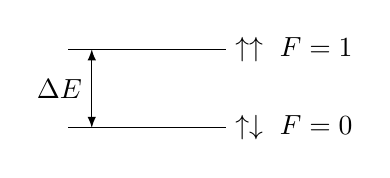
\begin{tikzpicture}
        \draw (0,0) -- (2,0) node[right]{$\uparrow\downarrow\ F=0$};
        \draw (0,1) -- (2,1) node[right]{$\uparrow\uparrow\ F=1$};
        \draw[>=latex, <->, black] (0.3,0) -- (0.3,1) node[left, pos=0.5]{$\Delta E$};
    \end{tikzpicture}
    \caption{Livelli iperfini dell'atomo di idrogeno.}
    \label{fig:livelli_iper}
\end{wrapfigure}
\noindent
 Il livello ad energia più bassa è quello con i due spin antiparallelo, quindi spin del protone e quello dell'elettrone opposto. In questo caso il momento angolare vale $F=0$. Mentre il livello con i due spin paralleli è quello con energia maggiore, in cui il momento angolare vale $F=1$. Quindi il livello più basso non è degenere e quello più alto sarà degenere con degenerazione pari a 3. Se l'atomo si trova nel livello più energetico e si diseccita emettendo un fotone, questo avrà un'energia $\Delta E = h\nu_0$ e facendo i conti si vede che
\[
    \nu_0 = 1.4204\um{GHz} \quad \Rightarrow \quad \lambda_0=21.105\um{cm}
\]
Quanto è probabile questa transizione? La transizione è proibita, quindi la probabilità di emissione spontanea è molto bassa. Infatti il coefficiente di Einstein di questa transizione vale 
\begin{equation}
    A_{10}=2.85\times10^{-15}\um{s}^{-1}.
    \label{eq:a10}
\end{equation}
Il tempo di dimezzamento del livello eccitato è invece molto lungo 
\begin{equation*}
    \tau_{1/2} = \frac{1}{A_{10}}\approx3.5\times10^{14}\um{s} \approx 1.1\times 10^7\um{yr}.
\end{equation*}
Ciò vuol dire che se siamo nel mezzo interstellare, un atomo di idrogeno viene eccitato da una collisione. Il fatto che il mezzo sia molto rarefatto fa sì che non si abbiano diseccitazioni per collisione ma soltanto dopo 11 milioni di anni (in media) avremo una diseccitazione radiativa. Le densità raggiungibili in laboratorio fanno sì che non sia possibile riprodurre il sistema, il che rende il mezzo interstellare un ambiente unico per lo studio di questi fenomeni.\\
Essendo la temperatura così bassa ($T\approx (80\div 100)\um{K}$), siamo sicuri di poter considerare il primo livello (quello eccitato degli iperfini) popolato?
\[
    T=300\um{K},\ kT=\frac{1}{40} \um{eV} \Rightarrow T=100\um{K},\ kT=\frac{1}{120} \um{eV} \gg\Delta E = 5.87\times 10^{-6}\um{eV}
\] 
L'energia termica è molto più grande dell'energia che separa i due livelli iperfini, quindi ci possiamo aspettare che sia popolato.\\
Facciamo una parentesi sull'LTE. Negli interni stellari possiamo considerare il plasma in condizioni di LTE. Ciò vuol dire che il popolamento relativo dei vari livelli energetici è governato dalle collisioni. Mi aspetto che al diminuire della densità, questo cessi di essere vero. Quando questo succede e quindi il nostro gas non è al LTE, bisogna risolvere le equazioni di rate dei processi che popolano e spopolano i livelli energetici. Se non vale LTE non possiamo considerare valide Boltzmann (quindi $\frac{n_2}{n_1}\neq\frac{g_2}{g_1}\exp{(-\frac{h\nu}{kT})}$) e non vale Kirchhoff (quindi $S_\nu \neq B_\nu(T)$). Vediamo cosa succede nel nostro caso specifico.\\
Si definiscono dei coefficienti, analoghi a quelli di Einstein per le reazioni, per le collisioni:
\begin{itemize}
    \item coefficiente di diseccitazione $\gamma_{21}$ tale che il rate di diseccitazione collisionale del livello due sia dato da $\gamma_{21}n_2n_e$.
    \item coefficiente di eccitazione $\gamma_{12}$ tale che il rate di eccitazione collisionale del livello due sia dato da $\gamma_{12}n_1n_e$
\end{itemize}
Immaginiamo di essere in una situazione in cui abbiamo un atomo a due livelli e di considerare sia i processi collisionali che quelli radiativi. Siamo in una condizione stazionaria in cui in media il numero di transizioni $1\to2 = 2\to1$. Il rate di eccitazione sarà dato da
\[
    n_1(B_{12}\Bar{J}+\gamma_{12}n_e)=n_2(A_{21}+B_{21}\Bar{J}+\gamma_{21}n_e)
\]
Vogliamo fare un ragionamento analogo a quello fatto a suo tempo per trovare le relazioni tra i coefficienti. Per farlo avevamo supposto LTE, ma le relazioni trovate restano comunque indipendenti da ciò. Analogamente faremo qui: assumeremo equilibrio termodinamico per calcolare le relazioni ma sappiamo che non c'è bisogno che sia verificato perché le reazioni siano vere.\\

\[
\text{LTE} \Rightarrow J_\nu = I_\nu =B_\nu(T)
\]
Siccome la funzione di Planck varia lentamente in termini di frequenza, nell'intervallo $\Delta\nu$ possiamo considerarla costante, quindi
\[
\Bar{J}\approx B_\nu(T)
\]
Inoltre, siccome siamo in LTE, possiamo scrivere
\[
    \frac{n_2}{n_1}=\frac{g_2}{g_1}e^{-\frac{h\nu}{kT}}
\]
Sostituiamo queste relazioni nelle equazioni di rate e otteniamo
\begin{equation}
    g_1\gamma_{12} = g_2 \gamma_{21} e^{-\frac{h\nu}{kT}}
    \label{rel-gamma}
\end{equation}
Consideriamo il mezzo interstellare. Gli atomi vengono eccitati collisionalmente e consideriamo il caso in cui il mezzo non viene illuminato, cioé consideriamo il caso in cui
\[
    \Bar{J} = 0
\]
Sostituiamo nelle equazioni di prima e otteniamo
\[
n_1 n_e \gamma_{12} =n_2(A_{21}+n_e\gamma_{21})
\]
\[
 \Rightarrow   \frac{n_2}{n_1}=\frac{\gamma_{12}n_e}{A_{21}+\gamma_{21}n_e}
\]
Sostituiamo la relazione tra $\gamma_{12}$ e $\gamma_{21}$ ottenuta in Eq. (\ref{rel-gamma}) e ottengo
\begin{equation*}
     \frac{n_2}{n_1}=\frac{g_2}{g_1}e^{-\frac{h\nu}{kT}}\frac{1}{1+\frac{A_{21}}{\gamma_{21}n_e}}    
\end{equation*}
Se non ci fosse l'ultimo termine avrei ottenuto la relazione di Boltzmann. Quando questo termine va a zero, il popolamento del livello è descritto dalla distribuzione di Boltzmann. Dire che questo termine va a zero implica
\begin{equation}
    \frac{A_{21}}{\gamma_{21}n_e}\ll 1 \Rightarrow A_{21} \ll n_e\gamma_{21}
    \label{eq:limite_bol}
\end{equation}
Cioè stiamo dicendo che, nel limite in cui la probabilità di diseccitazione radiativa diventa trascurabile rispetto a quella collisionale, ricadiamo nella distribuzionedi Boltzmann. Infatti sappiamo che in LTE il popolamento dei livelli è determinato dalle collisioni. \\
Quando vale la relazione Eq. (\ref{eq:limite_bol})? Quando si raggiunge una densità critica
\[
    n_{e,c} = \frac{A_{21}}{\gamma_{21}}
\]
Quando $n_e\gg n_{e,c} $ siamo in LTE, altrimenti no.\\
Per le transizioni permesse, il coefficiente $A_{21}$ sarà grande, quindi anche la densità critica mentre quella del mezzo sarà più piccola rispetto alla crititca. Non potremo quindi considerare il mezzo in LTE. Nel caso della reazione a 21cm abbiamo visto che $A_{21}$ è molto picocolo (Eq.(\ref{eq:a10})), e la densità critica vale
\begin{equation}
    \text{HI } 21\um{cm} \to n_c\approx3\times10^{-5}\um{cm}^{-3}
\end{equation}
Che è minore della densità delle nubi di HI ($\sim (1\div100)\um{cm}^{-3}$. Tuttavia riusciamo a vedere l'emissione delle nubi a 21 cm ma non riusciamo a farlo in laboratorio. Infatti in un qualsiasi laboratorio abbiamo densità molto più grandi rispetto a quella delle nubi. Inoltre in una nube abbiamo un'enorme quantità di atomi di idrogeno. Quindi per quanto sia un evento molto raro, questi due aspetti fanno sì che ci sia un'emissione che produce un segnale importante.\\
Ora vogliamo calcolare la riga di emissione spontanea dell'idrogeno neutro a 21 cm. Calcoliamo innanzitutto il popolamento dei livelli, cioè $n_2/n_1$
\[
\text{LTE} \Rightarrow     \frac{n_2}{n_1}=\frac{g_2}{g_1}e^{-\frac{h\nu}{kT}}
\]
Sappiamo che per $T=80K$, $h\nu = 5.87\times10^{-6}\um{eV}\ll kT=6.9\times10^{-3}\um{eV}$ e quindi che $e^{-\frac{h\nu}{kT}}\ll1$, il che implica che
\[
\frac{n_2}{n_1}\approx\frac{g_2}{g_1}=3
\]
L'ultima uguaglianza è dovuta al fatto che il livello 2 ha degenerazione uguale a 3, mentre il livello 1 non ha degenerazione, quindi è uguale a 1. Quindi, siccome le temperature tipiche delle nubi interstellari garantiscono un'energia termica che è diversi ordini di grandezza più grande della differenza di energia fra i livelli, il rapporto tra il popolamento dei livelli è indipendente dalla temperatura.\\
Sappiamo che 
\[
    \begin{cases}
        n_1+n_2 = n_\text{H}\\
        n_2/n_1=3
    \end{cases}
    \Rightarrow
    \begin{cases}
        n_1=\frac{n_\text{H}}{4}\\
        n_2=\frac{3}{4}n_\text{H}
    \end{cases}
\]
Abbiamo un mezzo rarefatto, vogliamo studiare l'emissione del mezzo non retroilluminato, quindi andiamo a riprendere la soluzione dell'equazione del trasporto 
\[
    I_\nu(\tau_\nu)=I_0(\nu)e^{-\tau_\nu}+\int_{0}^{\tau_\nu}e^{-(\tau_\nu-\tau_\nu')}S_\nu(\tau_\nu')d\tau_\nu'
\]
E dato che il mezzo non è retroilluminato $I_\nu(0)=0$. In caso di mezzo omogeneo avremmo 
\[
    I_\nu(\tau_\nu)=S_\nu(1-e^{-\tau_\nu})
\]
Ci aspettiamo che essendo rarefatto, il mezzo sia otticamente sottile
\[
    \tau_\nu\ll1\Rightarrow I_\nu(\tau_\nu) = j_\nu L
\]
Nel nostro caso non possiamo considerare il mezzo omogeneo, per cui
\[
    I_\nu(\tau_\nu)\approx \int j_\nu ds
\]
e abbiamo bisogno dell'intensità su tutto il profilo
\[
I=\int I_\nu d\nu = \int ds \int j_\nu d\nu
\]
In pratica, se conoscessimo la forma di $j_\nu$ potremmo calcolare l'intensità della riga. Ma in realtà possiamo calcolarlo, infatti 
\[
    j_\nu = \frac{h\nu_0}{4\pi}n_2A_{21}\Phi(\Delta \nu)
\]
E a questo punto lo sostituiamo e integriamo, ottenendo
\[
    I = \frac{h\nu_0}{4\pi}A_{21}\int n_2 ds
\]
Dove come al solito abbiamo sfruttato il fatto che $\int \Phi(\Delta \nu)d_\nu = 1$. Sapendo che $n_2=\frac{3}{4}n_\text{H}$, abbiamo
\[
    I = \frac{3}{16\pi}h\nu_0A_{21}\int n_\text{H} ds = \frac{3}{16\pi}h\nu_0A_{21} N_{\text{HI}}
    \label{eq:intemi}
\]
Con $N_\text{HI}$ densità di colonna dell'idrogeno neutro. È fondamentale osservare che l'intensità di emissione dipende dalla densità di colonna ma non dipende dalla temperatura! Ce lo aspettiamo poiché l'emissione spontanea dipende da $n_2$ che non dipende dalla temperatura. Il tutto perché $kT$ è enorme rispetto ad $h\nu$. Si fanno osservazioni nel radio, si misura l'intensità dalle righe, il coefficiente di Einstein lo conosciamo dalle misure di laboratorio e questo ci da una stima della densità di colonna. \\
Per caratterizzare completamente il mezzo ci sarebbe bisogno di misurare la densità della riga di assorbimento. Per farlo mettiamo una sorgente dietro il mezzo (\ref{fig:tralenubi}) e calcoliamo l'intensità:
\[
 I_\nu = I_\nu(0)e^{-\tau_\nu},
\]
con
\begin{equation}
    \tau_\nu = \int_{s_0}^{s}\alpha_\nu(s')ds'.
    \label{eq:prottica}
\end{equation}
Per caclcolare la profondità ottica dobbiamo conoscere il coefficiente di assorbimento
\[
    \alpha_\nu= \frac{h\nu}{4\pi}\Phi(\Delta\nu)\left[ n_1B_{12}-n_2B_{21}\right]
\]
Notare il termine dovuto all'emissione stimolata. Nelle bande ottiche lo abbiamo trascurato, poiché gli atomi del mezzo erano nel fondamentale e non c'erano atomi che potessero emettere nell'ottico con l'emissione stimolata. Qui conta e, come abbiao visto, possiamo riscriverlo come
\begin{equation}
    \alpha_\nu= \frac{h\nu}{4\pi}\Phi(\Delta\nu)n_1B_{12}\left[1 -e^{-\frac{h\nu}{kT}}\right]
    \label{eq:assorbimento}
\end{equation}
Nel visibile avevamo $h\nu$ grande rispetto a $kT$, ma a 21cm $h\nu\ll kT$, quindi $e^{-\frac{h\nu}{kT}}\approx 1-\frac{h\nu}{kT}$ e riscriviamo la \ref{eq:assorbimento} come
\begin{equation}
    \alpha_\nu= \frac{h\nu}{4\pi}\Phi(\Delta\nu)n_1B_{12}\frac{h\nu}{kT}
\end{equation}
Ora esprimiamo il coefficiente di assorbimento in termini di emissione spontanea sfruttando le relazioni
\begin{gather*}
    g_1B_{12}=g_2B_{21}\\
    A_{21}=\frac{2h}{c^2}\nu^3B_{21}\\
    n_1=\frac{n_\text{H}}{4}\\
    \frac{g_2}{g_1}=3
\end{gather*}
e otteniamo
\begin{equation}
    \alpha_\nu = \frac{3}{32\pi}\frac{hc^2}{kT}n_\text{H}A_{21}\frac{\Phi(\Delta\nu)}{\nu}
\end{equation}
A questo punto si ha la profondità ottica dalla \ref{eq:prottica} e otteniamo
\begin{equation}
    \tau_\nu = \frac{3}{32\pi}\frac{hc^2}{k}A_{21}\frac{\Phi(\Delta\nu)}{\nu}\int\frac{n_\text{H}}{T}ds
\end{equation}
Notiamo che la profondità ottica e quindi la riga di assorbimento dipendono anche dalla temperatura, a differenza della riga di emissione. Più alta è la temperatura più il mezzo è trasparente e più debole sarà la riga. \\
Con l'osservazione della riga a 21 cm si sono ottenute le prime evidenze che le nubi di gas non sono distribuite uniformemente sul disco ma a bracci di spirale.\\
\begin{figure}[t!]
    \centering
    \resizebox{.8\columnwidth}{!}{%
        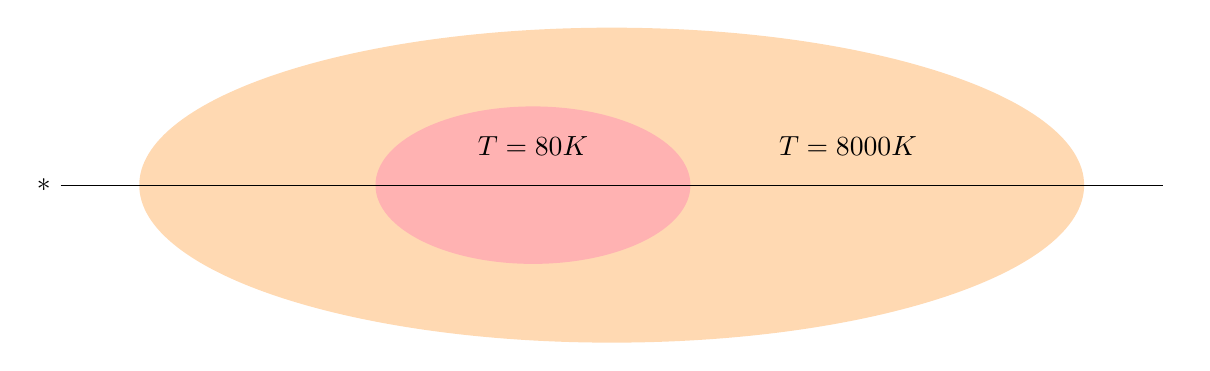
\begin{tikzpicture}
            \fill[orange!30] (0,0) ellipse (6 and 2);
            \fill[red!30] (-1,0) ellipse (2 and 1);
            \draw (-7,0) -- (7,0) node[left, pos=0]{$*$} node[right,pos=1]{$\text{\lateraleye}$};
            \node(hot) at (3,.5){$T=8000\um{K}$};
            \node(cold) at (-1,.5){$T=80\um{K}$};
        \end{tikzpicture}
    }
    \caption{Temperature delle nubi di idrogeno.}
    \label{fig:nubitemp}
\end{figure}
Lo studio della differente dipendenza da temperatura e densità nei casi di emissione ed assorbimento fece scoprire che oltre alla componente di idrogeno fredda ce ne fosse anche una calda (Fig.\ref{fig:nubitemp}). Il mezzo è composto per la maggior parte (in massa) dalla zona fredda, mentre la parte calda è molto rarefatta. La densità della zona fredda è circa $(1\div100)\um{cm}^{-3}$, mentre di quella calda è circa $(0.1\div1)\um{cm}^{-3}$.\\
\begin{figure}[b!]
    \centering
    \includegraphics[width=.4\columnwidth]{images/assoemi.png}
    \caption{Riga di emissione a 21 cm del mezzo interstellare nel (sopra) e la riga di assorbimento a 21 cm prodotta dal mezzo interstellare (sotto). Sorgente 3C 353.}
    \label{fig:assoemi}
\end{figure}
Un mezzo fatto come in Figura \ref{fig:nubitemp} produce righe di assorbimento ed emissione a 21 cm come nella Figura \ref{fig:assoemi}. Abbiamo visto nell'Eq. \ref{eq:intemi} che l'intensità della riga di emissione dipende solo dalla densità di colonna, quindi in particolare significa che è indipendente dalla temperatura. Quando andiamo ad osservare abbiamo che parte della riga sarà data dalla nube fredda e parte da quella calda. Se la densità di colonna lungo la linea di vista è confrontabile per il mezzo alle diverse temperature, la riga avrà due contributi che hanno intensità confontabile. Tuttavia la larghezza di questi contributi deve essere diversa: più larga in quella della zona calda, più stretta in quella della fredda. Ed è questo che notiamo guardando la Figura \ref{fig:assoemi}, in cui la riga di emissione ala base è larga e poi si stringe. è la sovrapposizione di due righe. Nella riga di assorbimento la situazione è diversa, dato che questa dipende dalla temperatura. Dato che la profondità ottica diminuisce con l'aumento della temperatura, l'intensità della riga di assorbimento prodotta nella zona calda sarà molto più debole di quella della zona fredda. Gran parte della riga è prodotta quindi nella zona fredda ed ha la larghezza di una riga ad $80\um{K}$ e non $8000\um{K}$.\\
Oltre a polvere ed idrogeno neutro, nel mezzo interstellare sono presenti delle nubi molecolari, le cui caratteristiche principali sono $n\approx 10^3\um{cm}^{-3}$, $T=10\div30\um{K}$. Queste sono composte principalmente da molecole di $\ce{H2}$. Sono difficili da osservare non avendo emissioni nel radio. Si possono osservare nell'ultravioletto se c'è una sorgente che le illumina. Per caratterizzarne la distribuzione geometrica non si usano le molecole di idrogeno, ma di molecole di $\ce{CO}$, anche queste abbastanza abbondanti. Queste hanno un'emissione molto intensa dovuta alle transizioni rotazionali a $\lambda =2.6\um{mm}$ che corrisponde a $\nu_0 = 115\um{GHz}$. Inoltre sono osservabili anche i multipli $2\nu_0,3\nu_0,\dots,n\nu_0$.\\
Una cosa interessante delle nubi molecolari è che si è scoperta la presenza di molecole di molti tipi diversi, tra cui anche molecole organiche (addirittura amminoacidi). E da queste molecole sono state scoperte intensità di emissione molto elevate che se fosse dovuta ad emissione termica per giustificarla avremmo bisogno di temperature di miliardi di gradi. In realtà si è scoperto che l'intensità così elevata non è da attribuire all'emissione termica ma all'inversione di popolazione dei livelli energetici che è più facile da ottenere per le molecole rispetto agli elementi. Si ha un'emissione non termica ma MASER. Nel cosmo ci sono molti fenomeni e molte molecole che producono MASER (OH, CH, SiO, $\ce{NH3}$, $\ce{H2O}$, HCN). Ciò che produce il pompaggio che determina l'inversione di popolazione è di solito un'intensa radiazione nell'infrarosso, a sua volta prodotta dalla polvere riscaldata da qualche tipo di processo (ad esempio, in scale piccole, nelle nubi stellari).